\documentclass{article}

% Language setting
% Replace `english' with e.g. `spanish' to change the document language
\usepackage[spanish]{babel}

\addto\captionsspanish{\renewcommand{\figurename}{Fig.}}

% Set page size and margins
% Replace `letterpaper' with `a4paper' for UK/EU standard size
\usepackage[letterpaper,top=2cm,bottom=2cm,left=3cm,right=3cm,marginparwidth=1.75cm]{geometry}

% Useful packages
\usepackage{amsmath}
\usepackage{graphicx}
\usepackage[colorlinks=true, allcolors=black]{hyperref}
\usepackage{float}
\usepackage[backend=biber,style=numeric]{biblatex}
\addbibresource{references.bib}

\begin{document}
\begin{titlepage}
    \centering
    % Logo
    \vspace*{1cm}
    
\includegraphics[width=0.4\linewidth]{logo-itba-site.png}
    \vspace{1.5cm}

    % Universidad
    {\Large Instituto Tecnológico de Buenos Aires \par}
    \vspace{1.5cm}

    % Título del trabajo
    {\Huge Trabajo Práctico Nro. 2: Autómatas Celulares \par}
    \vspace{1cm}

    % Materia
    {\LARGE Simulación de Sistemas (72.25)\par}
    \vspace{1.5cm}

    % Grupo
    {\large Grupo 2 \par}
    \vspace{0.8cm}

    % Integrantes
    {\large Máximo Chiatellino \par
    Federico Agustín Etchegorry \par
    Franco Morroni \par}
    \vfill

    % Fecha
    {\large 29 de agosto de 2025 \par}
\end{titlepage}


\clearpage
\tableofcontents
\clearpage


\section{Introducción}

Your introduction goes here! Simply start writing your document and use the Recompile button to view the updated PDF preview. Examples of commonly used commands and features are listed below, to help you get started.

Once you're familiar with the editor, you can find various project settings in the Overleaf menu, accessed via the button in the very top left of the editor. To view tutorials, user guides, and further documentation, please visit our \href{https://www.overleaf.com/learn}{help library}, or head to our plans page to \href{https://www.overleaf.com/user/subscription/plans}{choose your plan}.

\section{Modelo}

Se analiza un sistema de \(N\) partículas auto-propulsadas en un dominio cuadrado \([0,L]^2\) con condiciones de borde periódico (el plano se transforma en un toroide). Cada partícula avanza a módulo de velocidad constante \(v_0\) y está caracterizada por una orientación \(\theta_i(t)\). Estas partículas interactuan entre sí: cada partícula se alimenta de información con aquellas que se encuentran dentro de un disco de radio \(R_c\). Además, se adiciona otro elemento: el \textbf{ruido}, un valor aleatorio que perturba a las partículas alterando el ángulo con el que se trasladan. 

\subsection{Escenario I: Standard Vicsek Model (SVM) \cite{vicsek1995}}
El SVM representa el mecanismo de \emph{alineamiento promedio con ruido angular}. En cada paso temporal todas las partículas actualizan su orientación de forma sincrónica según:
\begin{enumerate}
  \item \textbf{Alineación de la dirección de movimiento:} la nueva dirección de una partícula (\(\theta(t+1)\)) es el ángulo promedio de las direcciones de los vecinos (incluida la propia partícula) dentro de \(R_c\), \(\langle\theta(t)\rangle_r\). Operativamente, esto equivale a tomar la dirección del vector suma de las velocidades unitarias de las partículas vecinas.
  \item \textbf{Ruido angular:} a esa dirección se le agrega un ruido (\(\Delta \theta\)) elegido con probabilidad uniforme en el rango de amplitud \([-\eta/2, \eta/2]\), que modela incertidumbre en la orientación.
\end{enumerate}
Tras fijar la orientación (\(\theta(t+1)= \langle\theta(t)\rangle_r + \Delta \theta\)), cada partícula avanza una distancia \(v_0\Delta t\) en su nueva dirección (\(x_i(t+1) = x_i(t) + v_0\Delta t\)) . Conceptualmente: el acoplamiento local tiende a \emph{coherenciar} las direcciones, mientras que el ruido los \emph{dispersa}. Al aumentar \(\eta\) (o disminuir \(\rho\)), el sistema transita de un estado globalmente ordenado (\(\langle v_a\rangle>0\)) a uno desordenado (\(\langle v_a\rangle\approx 0\)).

\subsection{Escenario II: Flocking con interacciones tipo votante \cite{baglietto2018}}
Este escenario implementa un mecanismo \emph{imitativo} en lugar del promedio vectorial. En cada paso:
\begin{enumerate}
  \item \textbf{Imitación local:} cada partícula selecciona al azar un solo vecino dentro de \(r\) y \emph{copia} su orientación instantánea.
  \item \textbf{Fluctuación:} puede añadirse un ruido angular pequeño de amplitud \(\eta\) para evitar estados absorbentes perfectos.
\end{enumerate}

\section{Implementación}

Cada simulación recibe como input dos archivos: el primero, estático, una lista con la cantidad de partículas (\( N\)), el largo y ancho de la grilla (\( L\)) y los radios de cada una de las partículas (\( r_c\)). El segundo input consta la lista de posiciones iniciales (\(\mathbf x_0\)) de cada una de las partículas junto con el ángulo inicial (\( \theta_0\) [rad]).

El output generado es un archivo binario que detalla para cada timestep (\(t_i\)), la posición de cada partícula \(\mathbf x_i(t)\) así como su velocidad  \(\mathbf v_i(t)\) y el ángulo de la partícula (\( \theta_i\)).

\section{Simulaciones}
  
Para el análisis se contará con unidades adimensionales. Para las distancias se empleará \texttt{u} que representa la unidad de longitud de la simulación. Cada paso temporal discreto será denominado \texttt{step}.

\subsection{Geometría}

El dominio de la simulación es una grilla de \(L\times L\) con condiciones de borde periódico, por lo que se comporta como un toroide.

\subsection{Parámetros y output}

Se listan a continuación los parámetros iniciales fijos de todas  las simulaciones:

\begin{itemize}
    \item La velocidad de las partículas se fija en \( v = 0.150 \) [u/step], encontrándose esta dentro del rango recomendado (Vicsek, 1995)
    \item Se simulan 2000 pasos para cada simulación. El estado inicial es  \( t_{min} = 0\) [step] mientras que el final es  \(t_{max} = 2000\) [step];
    \item Radio de interacción \(r_c\) = 1 [u]. 
    \item Radio de las partículas \(r\) = 0 [u]. 
\end{itemize}

\paragraph{Ruido a densidad fija:} Con \(\rho=2.5\) (combinaciones de \((N,L)\) más abajo), se grafica \(\eta\in[0,5]\) con \(\eta_i=0,2\times i\), \(i\in[0;25]\). Para cada \(\eta_i\) se ejecutan 5 réplicas independientes con posiciones (\(\mathbf x_0\)) y ángulos de las partículas (\( \theta_0\)) generados aleatoriamente para cada simulación.

\paragraph{Densidad a ruido fijo:} Con \(L=20\) y \(\eta=1\), se varía \(N_i=200\,i\), \(i \in [1,20]\), cubriendo \(\rho\in[0.5;10]\). También se realizanan 5 réplicas por condición con los mismos criterios.


\subsection{Observable}
El observable primario utilizado para determinar el orden colectivo se cuantifica con la \textbf{polarización} \(v_a\), el valor absoluto de la velocidad promedio normalizada.
\[
v_a(t) \;=\; \frac{1}{N v_0}\,\Big|\sum_{i=1}^N \mathbf v_i(t)\Big|\in[0,1],
\]
el \(v_a\) distingue el régimen desordenado (\(\approx 0\)) del polar (\(\approx 1\)). 

Se analiza cómo varía la polarización en función de la densidad y del ruido para cada uno de los dos modelos considerados. 

\subsubsection{Polarización y ruido}
Primero, se grafica el \(t\) vs \(v_a(t)\) para \(\eta \in [0;5]\) dado que se busca observar el comportamiento de \( \eta \) vs.\ \( v_a(t) \) promedio manteniendo la densidad constante para distintas combinaciones de \( L \) y \( N \).  Para cada una de las simulaciones con un determinado \(\eta_i\) se realizan 5 variantes. Para cada \(\eta_i\), se toman los últimos 400 pasos (el último 20\%) de \(v_a(t)\) de cada una de las 5 iteraciones (en total, \(5\times 400=2000\) valores) para estudiar el comportamiento del observable. Con ese conjunto agregado se calcula la media \(\mu_\eta\) y el desvío estándar \(\sigma_\eta\) donde \(v_{a_i}(t)\) denota la polarización en el paso \(t\) de la iteración \(i\):

\[
\mu_{\eta} \;=\; \frac{1}{2000}\,\sum_{i=0}^{4}\,\sum_{t=1601}^{2000} v_{a_i}(t)
\]

\[
\sigma_{\eta} \;=\; \sqrt{\frac{1}{2000}\,\sum_{i=0}^{4}\,\sum_{t=1601}^{2000}\Bigl(v_{a_i}(t)-\mu_{\eta}\Bigr)^2}
\]


Se analiza el comportamiento del sistema en los siguientes casos, para encontrar posibles variaciones en los resultados de acuerdo al \(N\) y \(L\) utilizados para calcular la densidad:
\begin{itemize}
    \item \(N=1000\) y \(L=20\) 
    \item \(N=500\) y \(L=14.142\)
    \item \(N=250\) y \(L=10\)
\end{itemize}

\subsubsection{Polarización y densidad}
A continuación, se conducen las simulaciones correspondientes para analizar   \(t\) vs \(v_a(t)\) (REFERENCIAR) para una serie  \(\rho\in [0;10]\). En este caso, se elige el ruido leve como parámetro fijo para analizar un comportamiento no determinístico.
Al igual que lo explicado para el análisis del ruido, se realizan 5 ejecuciones de la simulación para cada \(N_i\) y se elige el último 20\% de los valores de \(v_a(t)\) para el análisis. El cálculo de la media (\(\mu_N\)9 y el desvío estándar (\(\sigma_N)\) se realiza de la siguiente forma.

\[
\mu_{N} \;=\; \frac{1}{2000}\,\sum_{i=0}^{4}\,\sum_{t=1601}^{2000} v_{a_i}(t)
\]

\[
\sigma_{N} \;=\; \sqrt{\frac{1}{2000}\,\sum_{i=0}^{4}\,\sum_{t=1601}^{2000}\Bigl(v_{a_i}(t)-\mu_{N}\Bigr)^2}
\]



Se exhibe a continuación, para un escenario del Modelo Estándar de Vicsek específico, la transición del estado inicial de la simulación (Fig. ~\ref{fig:1}) al estado final (Fig. ~\ref{fig:2}), mostrando al inicio una distribución desordenada y, finalmente, llegándo a una distribución polar.
\begin{figure}[H]
    \centering
    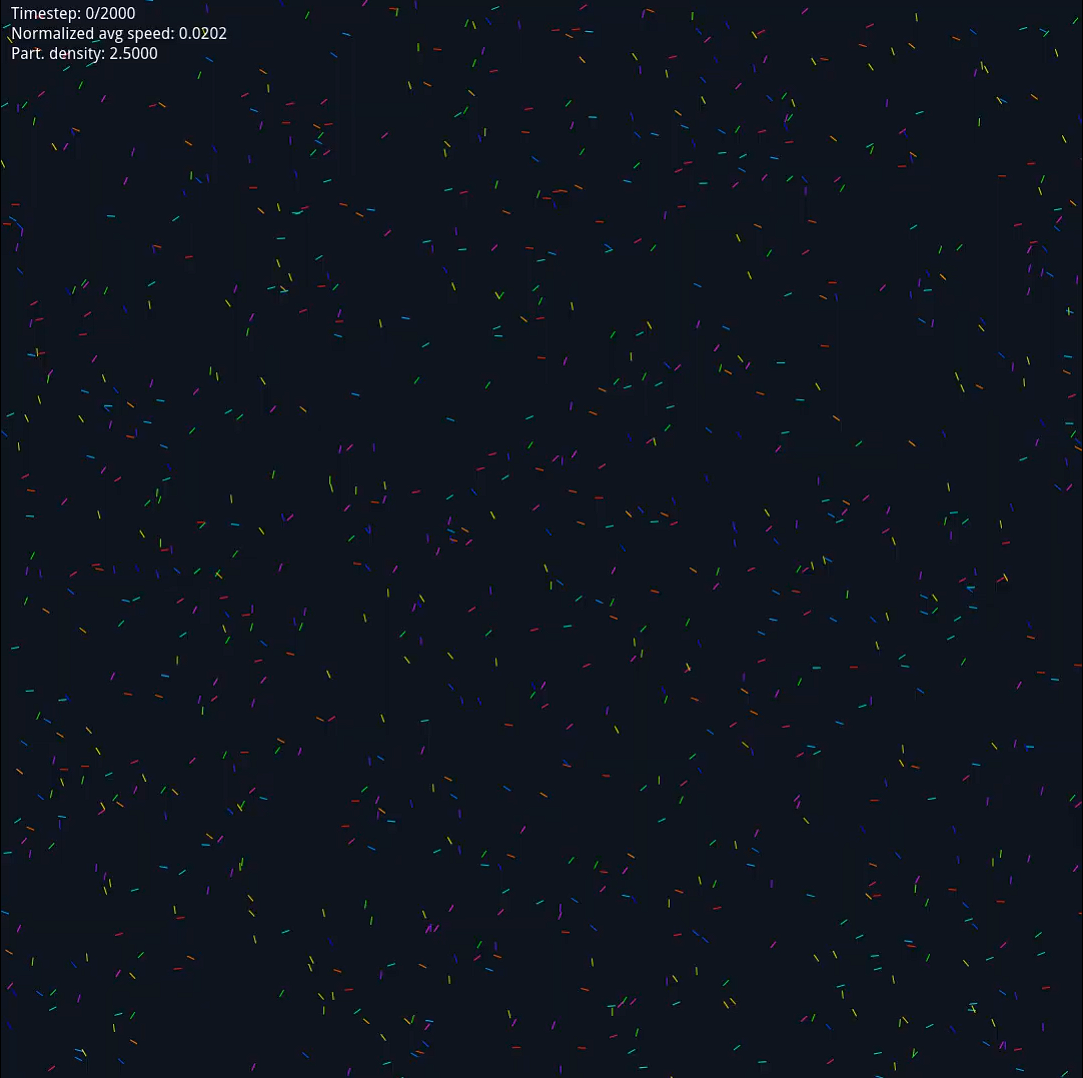
\includegraphics[width=0.75\linewidth]{simulation_example_t0.png}
    \caption{Simulación en el paso 0 (\(\eta=0, L=20, N=1000\)). El color de cada partícula indica el \(\mathbf v_i\)}
    \label{fig:1}
\end{figure}

\begin{figure}[H]
    \centering    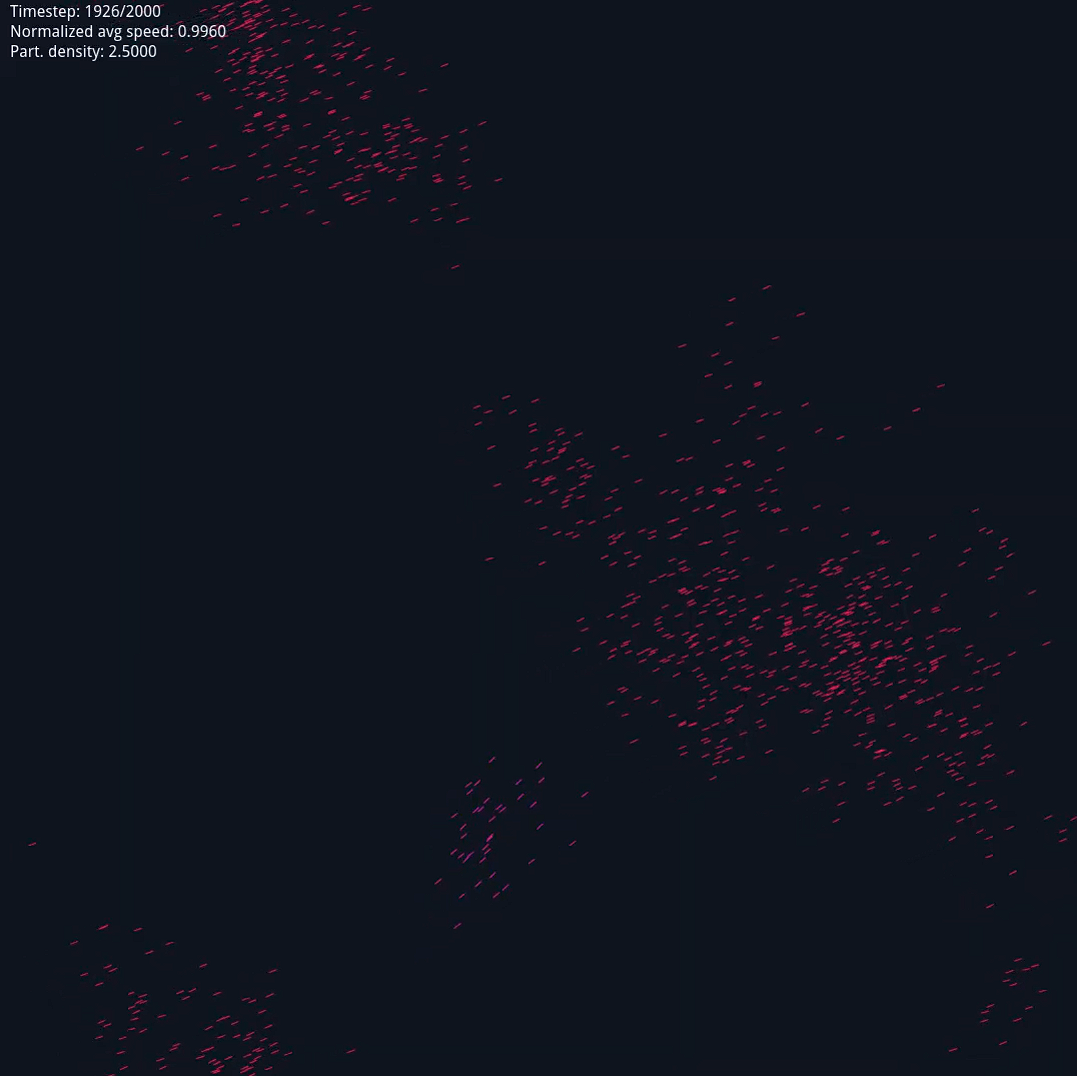
\includegraphics[width=0.75\linewidth]{animation_example.png}
    \caption{Simulación en el estado final (\(\eta=0, L=20, N=1000\))}
    \label{fig:2}
\end{figure}

\section{Resultados}

\subsection{Polarización y Ruido}
\subsubsection{Modelo Estándar de Vicsek}

Se presenta como varía la polarización en función del tiempo para los casos de \(\eta=0\) (Fig. ~\ref{fig:3}) y \(\eta = 5\) (Fig. ~\ref{fig:4}) con N=1000 y L =20. Se observa que, a medida que aumenta el ruido, disminuye la polarización. Con \(\eta=0\) se alcanza un estado estacionario polar en el paso 750, aproximadamente. Por otro lado, con \(\eta=5\) no se observa una tendencia a polarizarse. El valor de la polarización permanece relativamente constante a lo largo de toda la ejecución entre 0 y 0,1.
\begin{figure}[H]
    \centering
    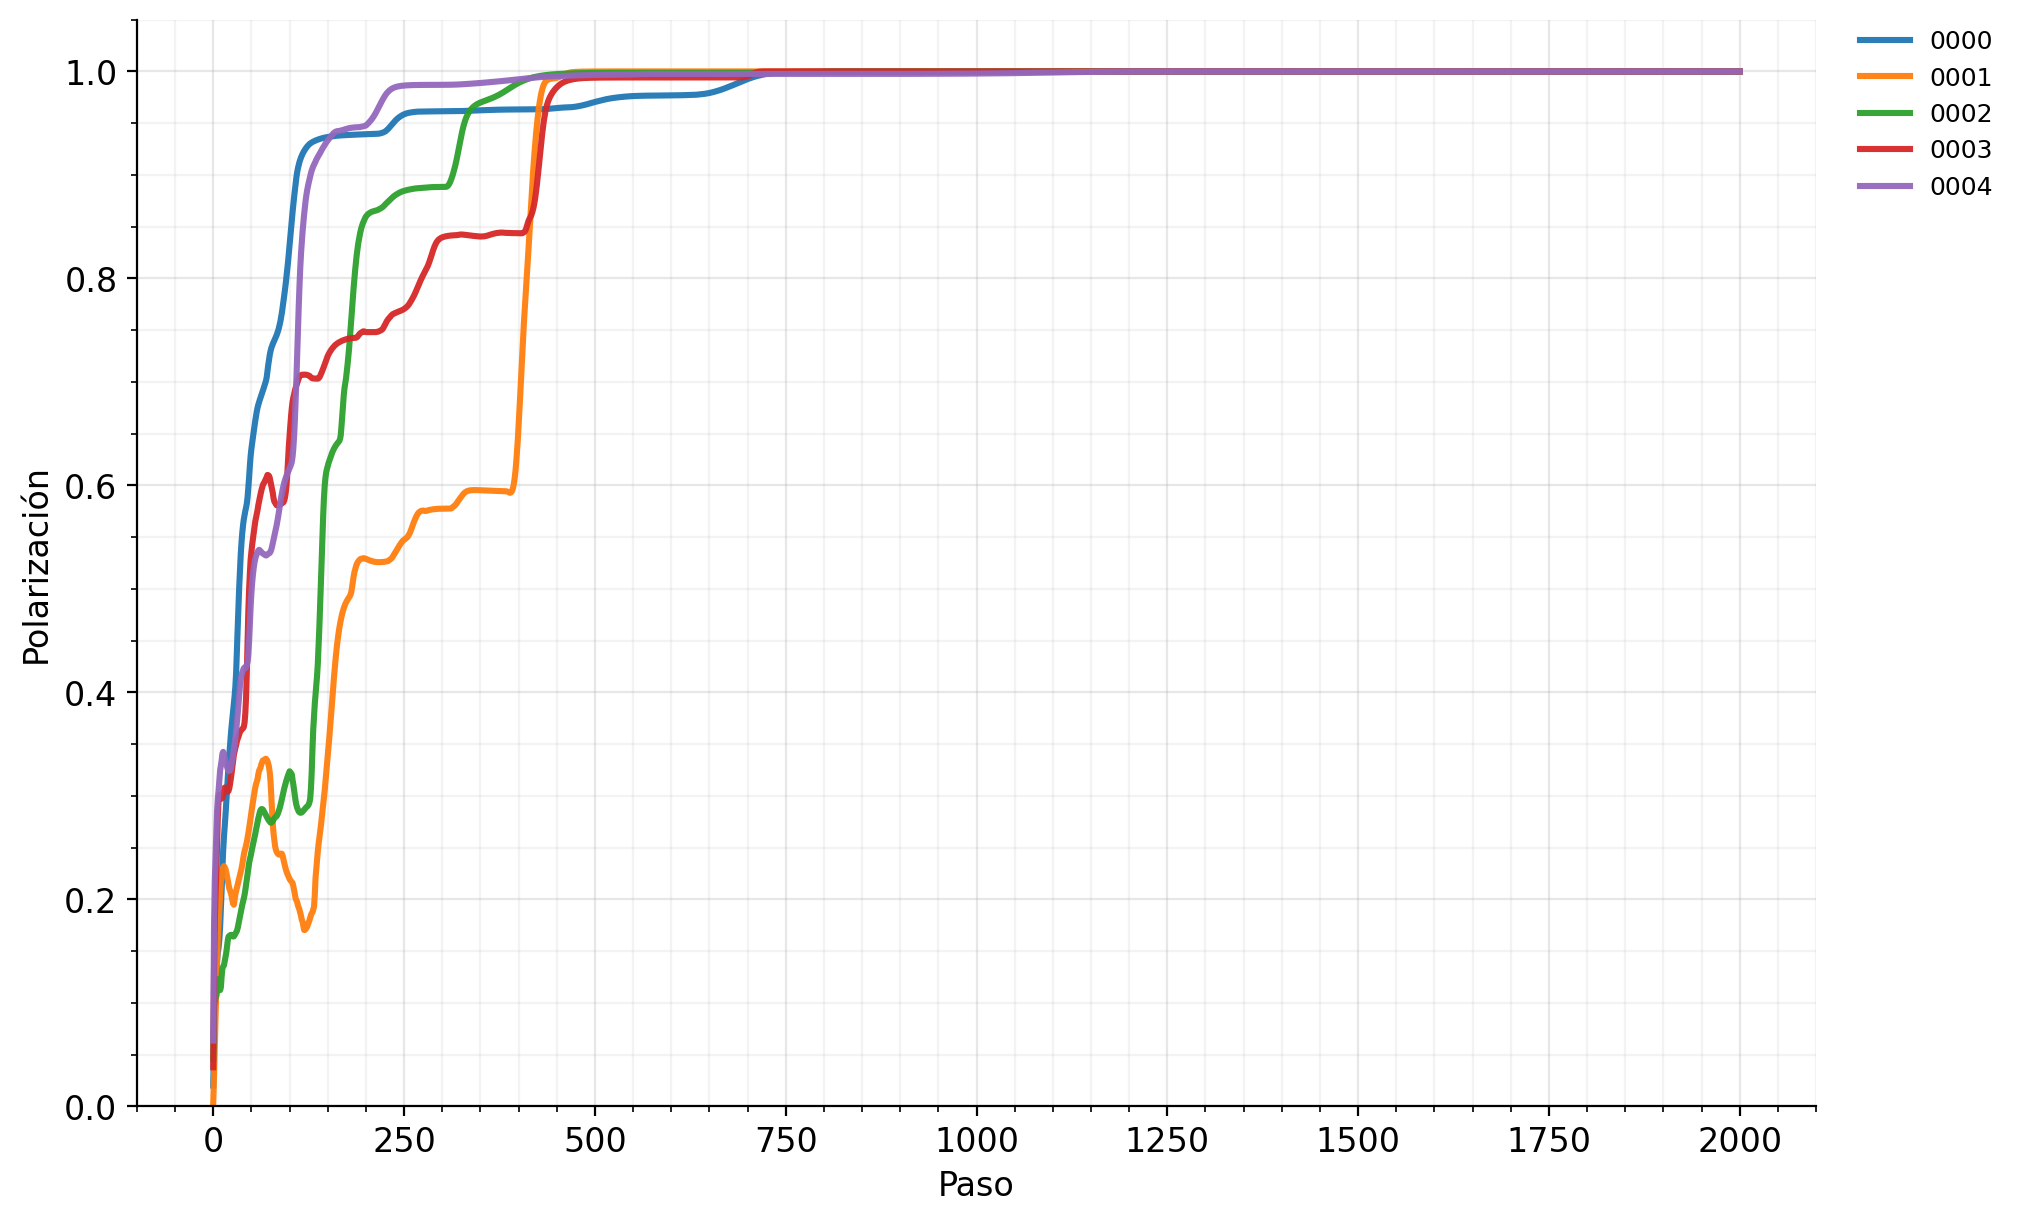
\includegraphics[width=1\linewidth]{noise_0_SVM.png}
    \caption{Paso vs. Polarización en el Modelo Estándar de Viscek con \(\eta =0\)}
    \label{fig:3}
\end{figure}

\begin{figure}[H]
    \centering
    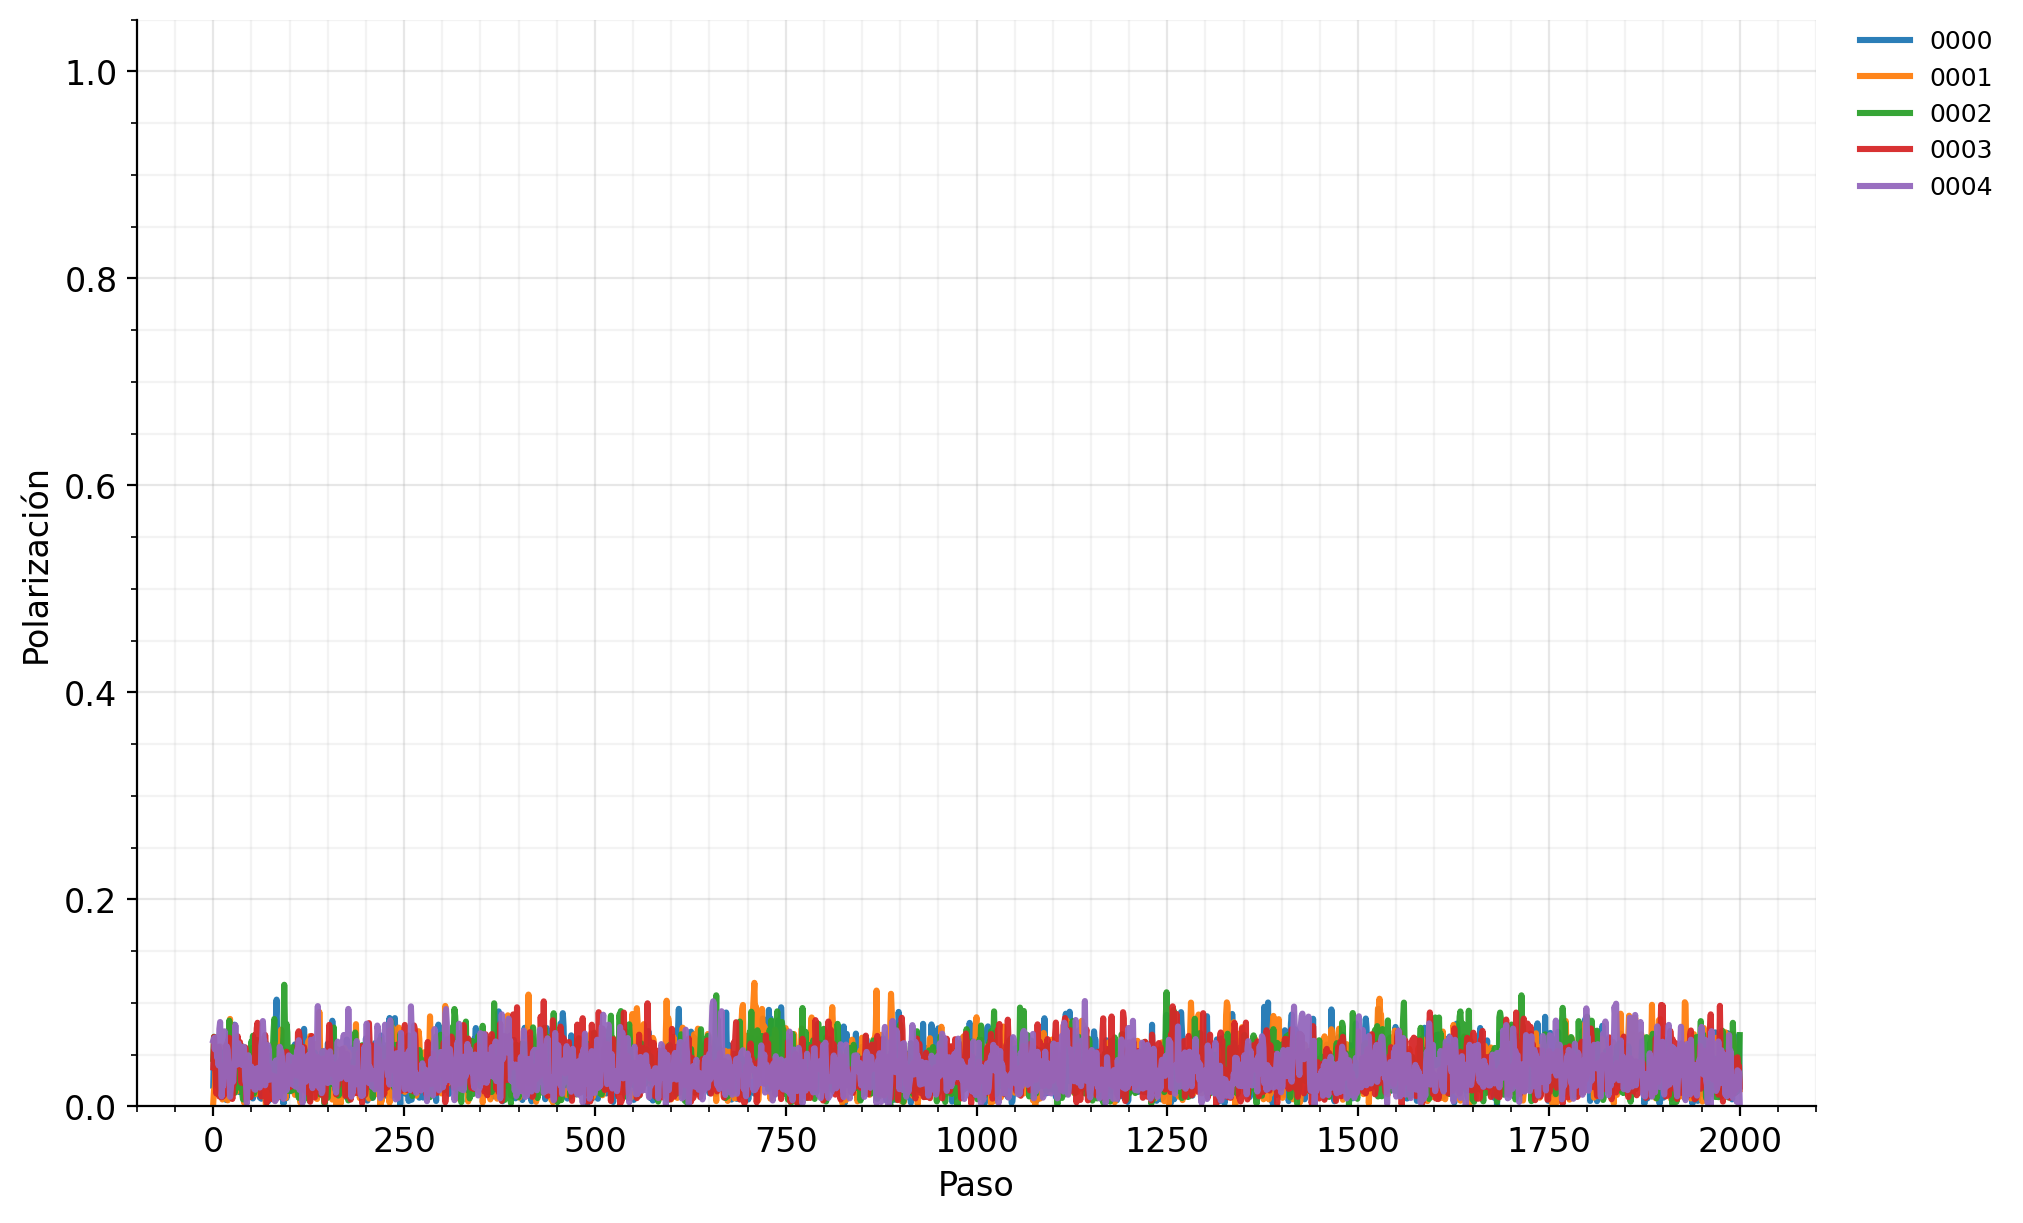
\includegraphics[width=1\linewidth]{noise_5_SVM.png}
    \caption{Paso vs. Polarización en el Modelo Estándar de Viscek con \(\eta = 5\)}
    \label{fig:4}
\end{figure}

Como ya se explicó en la sección de 'simulaciones' se grafica la relación \(\eta\) vs \(v_a\) promedio en el estado estacionario(Fig. ~\ref{fig:5}).

\begin{figure}[H]
    \centering
    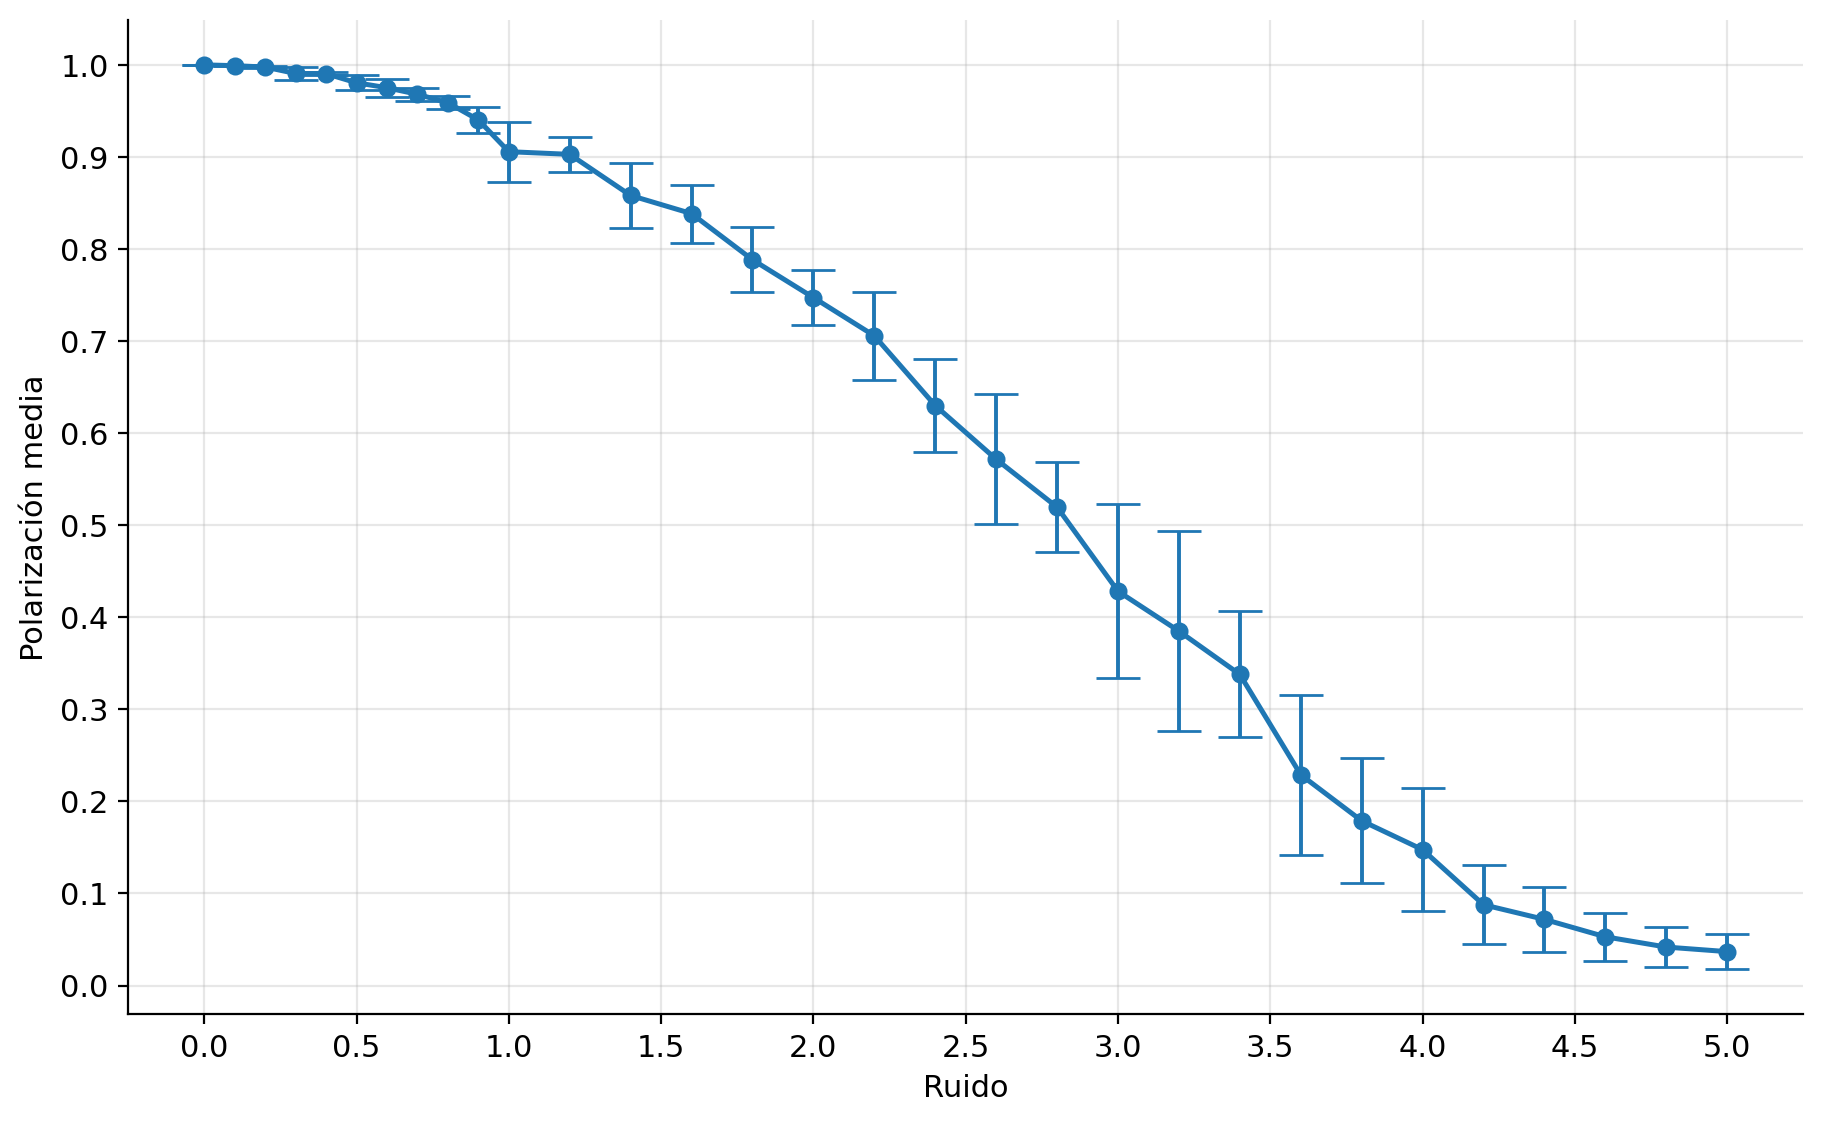
\includegraphics[width=1\linewidth]{noise_vs_polarization.png}
    \caption{Ruido vs Polarización media con L=20, N=1000}
    \label{fig:5}
\end{figure}

Los resultados muestran que la simulación es más polarizable mientras menor sea \(\eta\) y viceversa. Es interesante destacar que \(\sigma_{\eta}\) con los valores ruido intermedio (\(\eta \approx 3\)) muestran un desvío mucho mayor que los de los extremos. De acuerdo a las simulaciones realizadas, esto se debe a las oscilaciones en los valores de la polarización estacionaria (\(0.1\leq v_a\leq0.6\)).

Los resultados obtenidos se asemejan a lo expuesto en \cite{vicsek1995}
%"Novel Type of Phase Transition in a System of Self-Driven Particles" (Vicsek, 1994).




\subsubsection{Modelo de los Votantes }

A continuación, se presenta como se comporta la simulación cuando se emplea el modelo de los votantes para  \(\eta =0\)  y \(\eta =5\). Se observa que el tiempo medio de consenso es bastante 

\begin{figure} [H]
    \centering
    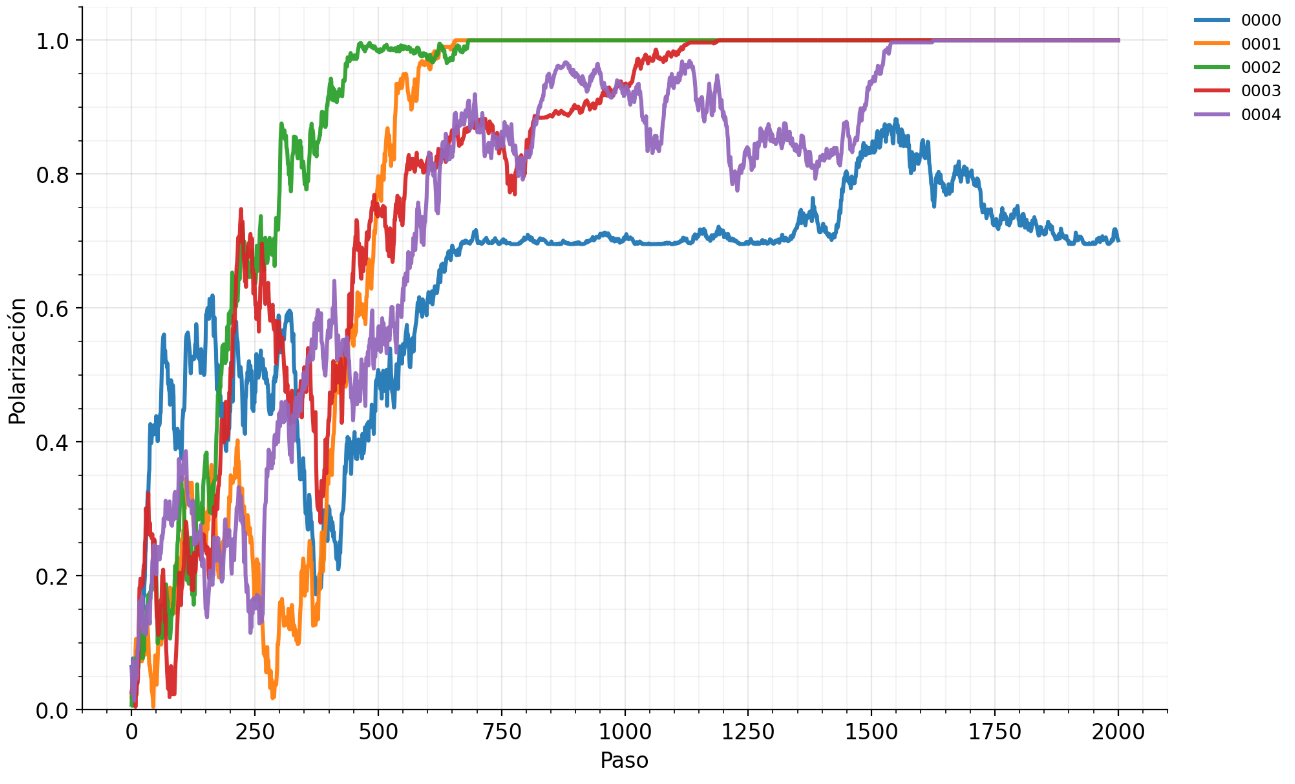
\includegraphics[width=1\linewidth]{noise_0_VM.png}
    \caption{Paso vs. Polarización en el Modelo de los Votante con \(\eta =0\)}
    \label{fig:placeholder}
\end{figure}
\begin{figure} [H]
    \centering
    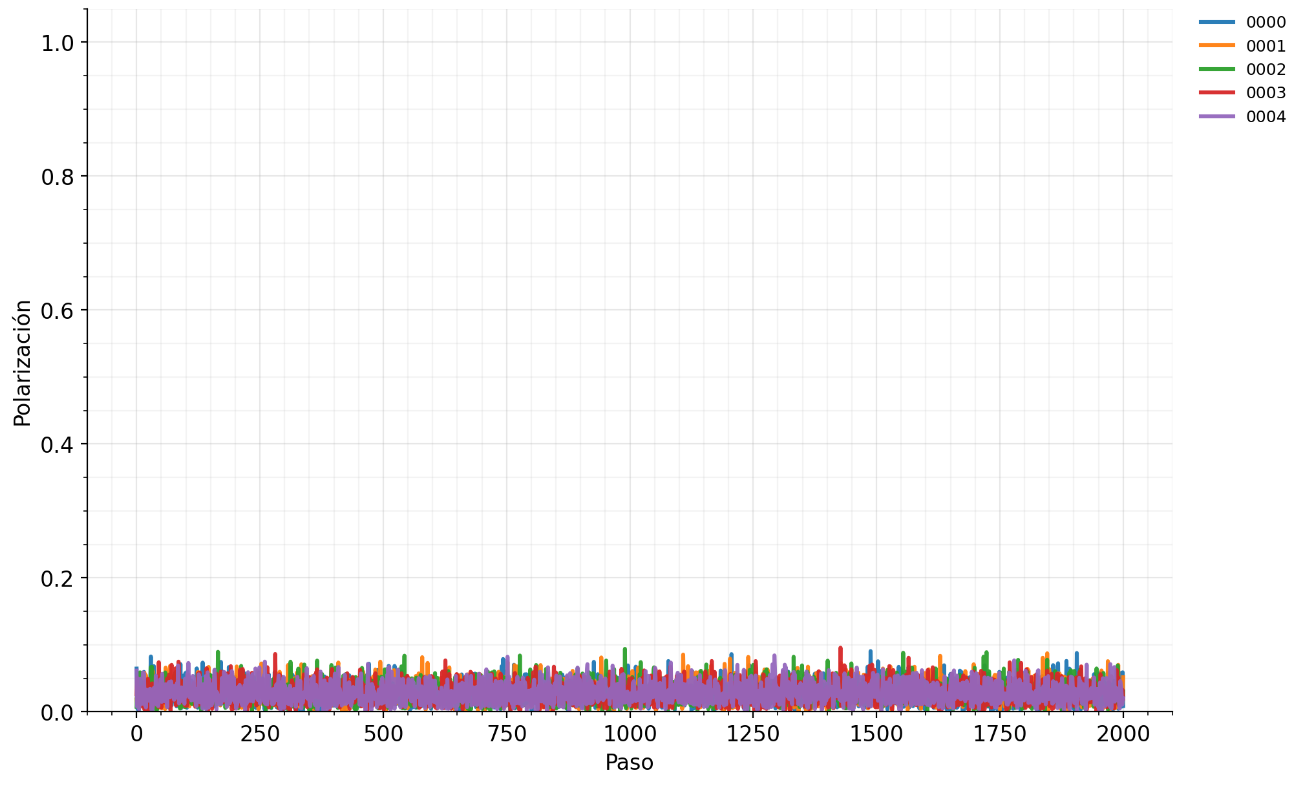
\includegraphics[width=1\linewidth]{noise_5_VM.png}
    \caption{Paso vs. Polarización en el Modelo de los Votante con \(\eta =5\)}
    \label{fig:placeholder}
\end{figure}

\section{Conclusiones}

En este trabajo se implementó y analizó un autómata off-lattice para simular bandadas de partículas autopropulsadas bajo dos modelos de interacción: el Modelo Estándar de Vicsek (SVM) y el modelo de interacciones tipo votante. A partir de las simulaciones realizadas, se obtuvieron los siguientes resultados principales:

\begin{itemize}
    \item La polarización \(v_a\) es un observable eficaz para caracterizar el orden colectivo del sistema, distinguiendo claramente entre estados desordenados (\(v_a \approx 0\)) y estados polarizados (\(v_a \approx 1\)).
    \item En el SVM, se confirmó que la polarización disminuye al aumentar el ruido \(\eta\) y aumenta con la densidad \(\rho\). El sistema alcanza un estado estacionario polar para valores bajos de \(\eta\) y densidades moderadas o altas.
    \item El modelo de interacciones tipo votante presenta transiciones más fluctuantes, reflejando la naturaleza estocástica de la imitación de un solo vecino. Esto evidencia que la forma de interacción local tiene un efecto significativo sobre la dinámica colectiva y el tiempo necesario para alcanzar el orden.
    \item El análisis de evolución temporal permitió establecer criterios claros para calcular el observable escalar en estado estacionario, considerando los últimos pasos de cada simulación y promediando sobre réplicas independientes para reducir la influencia del ruido inicial.
    \item Las curvas de input vs. observable escalar muestran que tanto el ruido como la densidad actúan como parámetros de control de la fase polar, corroborando hallazgos teóricos de Vicsek et al. (1995) y Baglietto \& Vázquez (2018).
\end{itemize}

En conjunto, estas simulaciones permiten visualizar y cuantificar la transición de un estado desordenado a uno ordenado en sistemas de partículas autopropulsadas, demostrando cómo distintos mecanismos de interacción y niveles de ruido afectan la dinámica colectiva. Este estudio sienta las bases para explorar variantes adicionales del modelo y comprender fenómenos de auto-organización en sistemas fuera del equilibrio.

\printbibliography[title={Referencias}]

\end{document}
